\section{Modelling} \label{sec:mod} % Incl. Subsection "Component Models"
The purpose of this section is to outline the model of the system. The model is intended to be used as a control model for minimizing the turbine fore-aft motion. The fore-aft motion dynamics of floating wind turbines are slow (a period of 30 seconds is normal) and the modelling is approached with this in mind: Dynamics which are relatively fast compared to the fore-aft motion dynamics are left out since they are of little importance to the control objective. In stead such components are modelled with algebraic equations. 

Modelling is approached from a component point of view where parts of the system are modelled individually. Each component takes a set of inputs and calculates a set of outputs. If the component contain dynamics they include internal states. Non-linear components are linearised individually at an operating point. Model parameters and operating points are extracted from Vestas Turbine Simulator (VTS) through the wtLin tool.


\subsection{wtLin component models}
A Matlab tool named wtLin has been developed by the LaC department in Vestas for creating a linear model based on simple component models and parameters extracted from VTS. The tool contains component models which can be connected in loops based on the input-output variables of each component model. A component can be in the form of mechanical models such as a generator or a converter but can also be models of other phenomena which are relevant for the system such as the interaction between the tower movement and the free wind.

The tool takes as input an operating point and a specific set of components. It outputs a connected linear model at that operating point.

In this section the relevant component models are derived. At the end the components are connected such that the flow of information in the model becomes apparent. 


\subsubsection{Drivetrain (stiff)}
As mentioned in \cref{sec:intro_wtcomponents} the drivetrain connects the rotor with the generator through a gearbox. In the simple stiff drivetrain model it is assumed that there is no dampening or spring effects in the drivetrain between the rotor and the generator. As such if some torque is applied at the rotor resulting in a change in twist angle at the rotor the resulting twist angle at the generator is instant and directly proportional to the twist angle at the generator.

The stiff drivetrain consists of two free inertias connected through a gearbox. The drivetrain is modelled from newtons second law for rotation as such:
\begin{equation}\label{eq:wtlin_comp_drivetrain}
	(J_{gL} + J_{r}) \ddot{\theta}_r = T_{r} + T_{g}
\end{equation}
The torques are related to the low-speed rotor side and thus the high-speed generator side inertias are mapped to the low speed side:
\begin{equation} \label{eq:wtlin_comp_inertiamap}
	J_{gL} = J_{gL} = J_{gH} \left(\dfrac{N_r}{N_g}\right)^2
\end{equation}
where $ N_r $ and $ N_g $ is the number of teeth on the rotor and generator side of the gearbox respectively. The rotor spins at angular velocity $ \dot{\theta}_r $.


\subsubsection{Drivetrain (flexible)}
A more accurate drivetrain model includes dampening and spring effects in the drivetrain between the rotor and the generator. The drivetrain is modelled with a dampener and a spring is between the rotor and the gearbox and between the gearbox and the generator. The model is then reduced by translating the dampener and spring from the generator side to the rotor side of the gearbox. As such the model ends up consisting of two inertias coupled through a spring with stiffness $ K $ and a dampener with dampening $ B $ where $ K $ and $ B $ are a combination of both the rotor and generator side dampener and spring coefficients. Due to the introduced spring and damper it is necessary to model both the rotor and and generator angle. \todo[]{Har Jesper modelleret drivetrain så at der også er fjeder og dæmper mellem gearbox og generator!?}

\begin{align} 
	J_{g} \ddot{\theta}_{gL} & = -B \dot{\theta}_{gL} + K(\theta_r - \theta_{gL}) - T_{g} \label{eq:wtlin_comp_drivetrain_flex_1} \\
	J_{r} \ddot{\theta}_r & = -B \dot{\theta}_{gL} -B - K(\theta_r - \theta_{gL}) + T_{r} \label{eq:wtlin_comp_drivetrain_flex_2}
\end{align}
\todo[inline]{I dæmper-termet. Skal det ikke være $ B(\dot{\theta_{gL}}-\dot{\theta_r}) $ eller lign?}
Recall that
\begin{align}
	\dot{\Omega} & = \ddot{\theta}_r \\
	\dot{\omega}_{L} & = \ddot{\theta}_{L} \\
	\dot{\theta}_g & = \omega \\
	\dot{\theta}_r & = \Omega
\end{align}
and
\begin{equation}\label{eq:wtlin_comp_drivetrain_flex_mod_3}
	\dot{\theta}_g = \left(\dfrac{N_g}{N_r}\right) \dot{\theta}_{gL} 
\end{equation}
Which leaves the full non-linear system model as:
%\begin{align} 
%	\dot{\omega}_{gL} & = \dfrac{-B \dot{\theta}_{gL} + K(\theta_r - \theta_{gL}) - T_{g}}{J_{g}} \label{eq:wtlin_comp_drivetrain_flex_mod_1} \\
%	\dot{\Omega} & = \dfrac{-B \dot{\theta}_{gL} -B - K(\theta_r - \theta_{gL}) + T_{r}}{J_{r}} \label{eq:wtlin_comp_drivetrain_flex_mod_2} \\
%\end{align}
\begin{align} 
	\dot{\omega} & = \dfrac{-B \left(\dfrac{N_r}{N_g}\right)\omega + K(\theta_r - \left(\dfrac{N_r}{N_g}\right) \theta_{g}) - T_{g}}{J_{g} \left(\dfrac{N_r}{N_g}\right) } \label{eq:wtlin_comp_drivetrain_flex_mod_1} \\
	\dot{\Omega} & = \dfrac{-B \left(\dfrac{N_r}{N_g}\right) \omega -B - K(\theta_r - \left(\dfrac{N_r}{N_g}\right) \theta_{g}) + T_{r}}{J_{r}} \label{eq:wtlin_comp_drivetrain_flex_mod_2} \\
	\dot{\theta}_g & = \omega \\
	\dot{\theta}_r & = \Omega
\end{align}
$ \omega $ and $ \Omega $ are the outputs while $ T_g $ and $ T_r $ are the inputs of the model.
	

\subsubsection{Generator model}
When considering the generator of a WT the obvious point of view (POV) is to consider it as outputting power when it is rotated. As such from this POV the input would be torque and rotational velocity and the output power would be the input to the converter. But with regards to rotor speed control the generator is on the contrary viewed as a source of torque. As such the inputs end up being rotational velocity and electrical power from the converter.

In Vestas' turbine simulator (VTS) the generator efficiencies are defined in tables and are dependent on grid output power $ P $ and generator speed $ \omega $. The output is three respective output efficiencies: 
\begin{enumerate}
	\item Mechanic efficiency: $ \eta_m(P,\omega) $
	\item Electric efficiency: $ \eta_e(P,\omega) $
	\item Auxiliary efficiency: $ \eta_a(P,\omega) $
\end{enumerate}
Where 
\begin{equation}\label{eq:wtLin_gen_effi}
	\eta(P,\omega) = \eta_m(P,\omega) + \eta_e(P,\omega) + \eta_a(P,\omega)
\end{equation}
From the total efficiency the output grid power is:
\begin{equation}\label{eq:wtLin_gen_elec_pow}
	P_{gen} \eta(P,\omega) = P
\end{equation}
where $ P_{gen} $ is the electrical power output of the generator.

This leaves the power loss from generator to grid to be defined as:
\begin{equation} \label{eq:wtLin_gen_pow_loss}
	P_{loss}(P, \omega) = P_{gen} - P = \dfrac{P}{\eta(P, \omega)} - P
\end{equation}
The power of a rotating machine can be defined as the product of torque and rotational velocity:
\begin{equation}\label{eq:wtLin_power_in_rot}
	P_{gen} = T_{gen} \omega
\end{equation}
As such for the system at hand the torque can be defined by rearranging \cref{eq:wtLin_power_in_rot} and substituting in $ P_{gen} $ from \cref{eq:wtLin_gen_pow_loss}. This leaves the non-linear generator model to be:
\begin{equation}\label{key}
	T_{gen}(P, \omega) = \dfrac{P_{loss}(P, \omega) + P}{\omega}
\end{equation}
From \cref{eq:wtLin_gen_pow_loss} it is visible that $ P_{loss}(P,\omega) $ is dependent on $ \eta(P, \omega) $. The $ \eta $ function is extracted from VTS and linearized.

The linear model of the generator is gained through a taylor expansion. The notation is relaxed a bit such that $ P_{loss}( P, \omega) $ is simply expressed as $ P_{loss} $. It is assumed that the system is linearised around an operating point and thus the $ T_{gen}(P_o, \omega_o) $ part is equal to zero.
\begin{equation}\label{eq:wtLin_taylor}
	T_{gen}( P, \omega) \approx T_{gen}(P_o, \omega_o) + 
	\left. \dfrac{\partial T_{gen}( P, \omega)}{\partial P} \right |_{P_o,\omega_o} ( P-P_o) + 
	\left. \dfrac{\partial T_{gen}( P, \omega)}{\partial \omega} \right |_{P_o,\omega_o} (\omega - \omega_o)
\end{equation}
Below the the generator torque sensitivity to the grid power change term from \cref{eq:wtLin_taylor} is derived. From \cref{eq:wtLin_gen_1_1} to \cref{eq:wtLin_gen_1_2} the \textit{sum rule} is used to split the derivative. From \cref{eq:wtLin_gen_1_2} to \cref{eq:wtLin_gen_1_3} the first fractions in the denominators of the partial derivatives of the two terms are treated as a product of two functions thus the \textit{product rule} is used. The assumption is that the grid power is completely disconnected from the generator through the converter. Thus from \cref{eq:wtLin_gen_1_3} to \cref{eq:wtLin_gen_1_4} $ \, \dfrac{\partial \, \omega^{-1}}{\partial P} = 0 $.
\begin{align} 
	\dfrac{\partial T_{gen}( P, \omega)}{\partial P} &= \dfrac{\partial \left (\dfrac{P_{loss} +  P}{\omega}\right )}{\partial P} \label{eq:wtLin_gen_1_1} \\
	& = \dfrac{\partial \left (\dfrac{P_{loss}}{\omega} \right )}{\partial P} + \dfrac{\partial \left ( \dfrac{ P}{\omega} \right )}{\partial P} \label{eq:wtLin_gen_1_2} \\
	& = \dfrac{1}{\omega} \cdot \dfrac{\partial P_{loss}}{\partial P} + \dfrac{\partial \left ( \dfrac{1}{\omega} \right )}{\partial P} P_{loss} + \dfrac{1}{\omega} \cdot \dfrac{\partial P}{\partial P} + \dfrac{\partial \left (\dfrac{1}{\omega} \right )}{\partial P}  P \label{eq:wtLin_gen_1_3} \\
	& = \dfrac{1}{\omega} \cdot \dfrac{\partial P_{loss}}{\partial P} + \dfrac{1}{\omega} \label{eq:wtLin_gen_1_4}
\end{align}


The generator torque sensitivity to rotational velocity change from \cref{eq:wtLin_taylor} is then derived:
\begin{align}
	\dfrac{\partial T_{gen}(P, \omega)}{\partial \omega} & = \dfrac{\partial \left (\dfrac{P_{loss} +  P}{\omega}\right )}{\partial \omega} \\
	& = \dfrac{\partial \left (\dfrac{P_{loss}}{\omega} \right )}{\partial \omega} + \dfrac{\partial \left (\dfrac{P}{\omega} \right )}{\partial \omega} \\
	& = \dfrac{1}{\omega} \cdot \dfrac{\partial P_{loss}}{\partial \omega} + \dfrac{\partial \left (\dfrac{1}{\omega} \right)}{\partial \omega} P_{loss} + \dfrac{1}{\omega} \dfrac{\partial P}{\partial \omega} + \dfrac{\partial \left (\dfrac{1}{\omega} \right )}{\partial \omega} P \\
	& = \dfrac{1}{\omega} \cdot  \dfrac{\partial P_{loss}}{\partial \omega} - \dfrac{1}{\omega^2}(P + P_{loss}) + \dfrac{1}{\omega} \dfrac{\partial P}{\partial \omega} \\
	& = -\dfrac{1}{\omega^2}(P + P_{loss}) + \dfrac{1}{\omega} \cdot \dfrac{\partial P_{loss}}{\partial \omega}
\end{align}
The above derived generator model is referred to the low-speed generator side by replacing $ \omega $ with $ \omega_L $ where $ \omega_L = \left (\dfrac{N_r}{N_g} \right ) \omega $. This yields the final linear generator model evaluated at the operating point $ (P_o, \omega_o) $. Furthermore $P_{loss}$ is still just a function of $ \omega_L $ and $ P $:
\begin{equation}
	\begin{split}
		T_{gen}(P, \omega_L) 	& \approx \left. \left ( \dfrac{1}{\omega_L} \cdot \dfrac{\partial P_{loss}(P, \omega)}{\partial P} + \dfrac{1}{\omega_L} \right ) \right |_{P_o,\omega_{L_o}} (P - P_0) \\ 
		& + \left ( -\dfrac{1}{\omega_L^2}(P + P_{loss}(P, \omega)) + \left. \dfrac{1}{\omega_L} \cdot \dfrac{\partial P_{loss}(P, \omega)}{\partial \omega_L} \right ) \right |_{P_o,\omega_{L_o}} (\omega_L - \omega_{L_o})
	\end{split}
\end{equation}


Presently the generator model in wtLin is implemented assuming a stiff drivetrain such that $ \Omega = \omega_L $ and as such the input to the generator model is $ \Omega $.  \todo[]{Er det muligt at ændre modellen så at den tager højde for et flexibelt drivetrain? Giver det overhovedet mening?}


\subsubsection{Unity model converter} \label{sec:wtLin_conv_unity}
The converter is regarded as a source of electrical power whose output is the power which is input to the generator.

The dynamics of modern converters are way faster than the rotor and tower dynamics and therefore it is simply modelled as an algebraic equation as a direct feed-through:
\begin{equation}\label{eq:wtLin_comp_convdft}
	P_{conv} = P_{ref}
\end{equation}
In other words the converter is treated as a \textit{black box} system which, when given a power reference, delivers a power equal to said power reference instantly.


\subsubsection{Aerodynamic torque} \label{sec:wtLin_aero_torque}
In \cref{sec:theory_aero} the rotor torque was defined for a blade by integrating over the torque component of each blade element based on a combination of the lift and drag forces. When calculating the total stationary torque it is convenient to use the pre-calculated power coefficient values $ C_P $ to determine the torque \cite{Knudsen2013}.

In \cref{eq:power_w_Cp} the extractable power from the free wind was defined. When combining this equation with the definition of power in a mechanical system the torque on the rotor can be expressed:
\begin{equation}\label{eq:wtLin_Mrot_lambda}
	M_{rot}(\Omega, \lambda) = \dfrac{1}{2} \rho A_d v_0^3 \, C_p(\theta, \lambda) \dfrac{1}{\Omega}
\end{equation}
$ C_P $ is the power coefficient and table lookups of it are extracted from VTS.

The TSR is dependent on $ \Omega $ and $ v_0 $ and thus the rotor torque model ends up being dependent on $ \theta $, $ \Omega $ and $ v_0 $:
\begin{equation}\label{eq:wtLin_Mrot_wind}
	M_{rot}(\theta, \Omega, v_0) = \dfrac{1}{2} \rho A_d v_0^3 \, C_p(\theta, \Omega, v_0) \dfrac{1}{\Omega}
\end{equation}
The model is then linearised at an operating point $ (\theta_o, \Omega_o, v_{0_o}) $:
\begin{align}
	M_{rot}(\theta, \Omega, v_0) \approx M_{rot}(\theta_o, \Omega_o, v_{0_o}) 
	& + \left. \dfrac{\partial M_{rot}(\theta, \Omega, v_0)}{\partial \theta} \right |_{\theta_o, \Omega_o, v_{0_o}} ( \theta-\theta_o) \\
	& + \left. \dfrac{\partial M_{rot}(\theta, \Omega, v_0)}{\partial \Omega} \right |_{\theta_o, \Omega_o, v_{0_o}} ( \Omega-\Omega_o) \\
	& + \left. \dfrac{\partial M_{rot}(\theta, \Omega, v_0)}{\partial v_0} \right |_{\theta_o, \Omega_o, v_{0_o}} ( v_0 - v_{0_o})
\end{align}


\subsubsection{Aerodynamic thrust} \label{sec:wtLin_aero_thrust}
In \cref{sec:wtLin_aero_torque} the stationary rotor torque was calculated based on the pre-calculated power coefficient table. Likewise the stationary rotor thrust can be calculated from the pre-calculated thrust table $ C_T $. Thus the model of the stationary aerodynamic rotor thrust force ends up being:
\begin{equation} \label{eq:wtLin_aero_thrust}
	F_T = \dfrac{1}{2} A \rho A_d v_0^2 C_T(\theta, \Omega, v_0)
\end{equation}
Just like for $ C_P $, table lookups of $ C_T $ are extracted from VTS. $ C_T $ like $ C_P $ is a mapping from the pitch angle, rotor velocity and free wind speed to a total stationary rotor thrust.


\subsubsection{Rotor wind}
There is an interaction between the tower fore-aft movement and the wind speed which ultimately results in a constantly changing wind speed as seen from the rotor's POV. Thus it is necessary to calculate the \textit{free} wind speed as observed from the rotors point of reference. This is simply done by subtracting the free wind speed $ v_0 $ from the hub translational velocity $ v_y $.
\begin{equation}\label{eq:wtlin_comp_rotorwind}
	v_{0_{rot}} = v_{0} - v_y
\end{equation}
$ v_{0_{rot}} $ is \underline{not} the rotor wind which is the wind speed at the rotor plane but the free wind modified by the turbine velocity.


\subsubsection{Fore-aft tower model}
The fore-aft motion is both the \textit{surge} and \textit{pitch} motion of turbine structure. In most literature the DOF notation seen is as seen in \cref{fig:fowt_coordinates}. This notation will hereinafter be denoted the \textit{"normal DOF notation"}. Vestas uses another notation which will be denoted the \textit{Vestas DOF notation}: Most importantly \textbf{x} and \textbf{y} are interchanged and surge in the normal DOF notation is called \textit{tilt} in Vestas DOF notation. This document for the most part adopts the normal DOF notation and one is thus directed to \cref{fig:fowt_coordinates} if in doubt about which movement is the subject of discussion.

The fore-aft tower motion is both the surge direction translation and the pitch angle rotation. The fore-aft movement is modelled by a mass-spring-damper system:
\begin{equation}\label{eq:wtlin_comp_fore-aft_ay1}
	\ddot{p}_y T = F_{rot} - F_d + F_s
\end{equation}

when isolating $ \ddot{p}_y $ this becomes:
\begin{equation}\label{eq:wtlin_comp_fore-aft_ay2}
	\ddot{p}_y = \dfrac{F_{rot} - B \dot{p}_y + K p_y}{T}
\end{equation}
We then define:
\begin{align}
	\dot{v}_y & = \ddot{p}_y \label{eq:wtlin_comp_fore-aft_ay} \\
	\dot{p}_y & = v_y \label{eq:wtlin_comp_fore-aft_vy}
\end{align}
which yields the fore-aft tower model:
\begin{align}
	\dot{v}_y & = \dfrac{F_{rot} - B v_y + K p_y}{T}  \label{eq:wtlin_comp_fore-aft_1} \\
	\dot{p}_y & = v_y \label{eq:wtlin_comp_fore-aft_2}
\end{align}


\subsubsection{Side-side tower model}



\subsubsection{Pitch system dynamics} \label{sec:mod_wtLin_pitch}
The pitch system dynamics are modelled with a simple first order low-pass filter which in the frequency domain looks like such:
\begin{equation}\label{eq:wtLin_pitch_freq}
	\theta(s) = \dfrac{1}{\tau_{pit} s + 1} (\theta_{ref}(s) + \theta_{fatd}(s))
\end{equation}
In the time domain this model is:
\begin{equation}\label{eq:wtLin_pitch_time}
	\dot{\theta} =\dfrac{(\theta_{ref}(s) + \theta_{fatd}(s)) - \theta}{\tau_{pit}}
\end{equation}

% The calculation of the time-domain version:
%\begin{align}\label{eq:wtLin_pitch}
%	\theta(s) & = \dfrac{1}{\tau_{pit} s + 1} (\theta_{ref}(s) + \theta_{fatd}(s)) \\
%	(\tau_{pit} s + 1) \theta(s) & = (\theta_{ref}(s) + \theta_{fatd}(s)) \\
%	\tau_{pit}\theta s + \theta(s)  & = (\theta_{ref}(s) + \theta_{fatd}(s)) \\
%	\tau_{pit}\dot{\theta} + \theta  & = (\theta_{ref}(s) + \theta_{fatd}(s)) \\
%	\dot{\theta} & =\dfrac{(\theta_{ref}(s) + \theta_{fatd}(s)) - \theta}{\tau_{pit}}
%\end{align}


The inputs are the pitch angle reference $ \theta_{ref} $ and the fore-aft tower dampener contribution $ \theta_{fatd} $ and the output is the pitch system pitch angle.


\subsubsection{Full Load Controller (FLC)} \label{sec:mod_wtLin_FLC}
The FLC is a PI controller on the form seen in \cref{fig:PIcontroller}.
\begin{figure}[h]
	\centering
	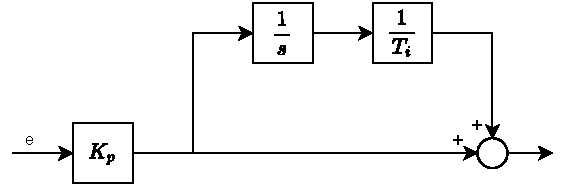
\includegraphics[width=0.5\linewidth]{Graphics/PiController.pdf}
	\caption{Block diagram of the PI controller on the \textit{$T_i$} form}
	\label{fig:PIcontroller}
\end{figure}
The controller model is therefore:
\begin{equation}\label{eq:wtlin_comp_flc_1}
	\theta_{ref}(s) = (K_{p \theta} + K_{p \theta} \dfrac{1}{T_{i \theta} s}) e(s)
\end{equation}
which is reduced to the form:
\begin{equation}\label{eq:wtlin_comp_flc_1}
	\theta_{ref}(s) = K_{p \theta}\dfrac{T_{i \theta} s + 1}{T_{i \theta} s} e(s)
\end{equation}
Gain scheduling is present in the turbine controller and the specific gain scheduling value is applied based on the operating point:
\begin{equation}\label{eq:wtlin_comp_flc_3}
	\theta_{ref}(s) = K_{gs \theta} K_{p \theta} \dfrac{T_{i \theta} s + 1}{T_{i \theta} s} e(s)
\end{equation}

In the time domain FLC controller is then represented as:
\begin{align}
	\theta_{ref}(s) & = K_{gs \theta} K_{p \theta} \dfrac{T_{i \theta} s + 1}{T_{i \theta} s} e(s) \\
	\theta_{ref}(s) & = K_{gs \theta} K_{p \theta} (\dfrac{T_{i \theta} s}{T_{i \theta} s} + \dfrac{1}{T_{i \theta} s}) e(s) \\
	\theta_{ref}(s) & = K_{gs \theta} K_{p \theta} e(s) +  K_{gs \theta} K_{p \theta} \dfrac{1}{T_{i \theta} s}e(s) \\
	\theta_{ref}(s) s & = K_{gs \theta} K_{p \theta} e(s) s +  K_{gs \theta} K_{p \theta} \dfrac{1}{T_{i \theta}}e(s) \\
	\dot{\theta}_{ref} & = K_{gs \theta} K_{p \theta} \dot{e} +  K_{gs \theta} K_{p \theta} \dfrac{1}{T_{i \theta}}e
\end{align}



\subsubsection{Partial Load Controller (PLC)}
The PLC is a PI-controller on the same form as the \hyperref[sec:mod_wtLin_FLC]{\textbf{FLC}} controller:
\begin{equation}\label{eq:wtlin_comp_flc}
	P_{ref}(s) = K_{gs P} K_{p P} \dfrac{T_{i P} s + 1}{T_{i P} s} e(s)
\end{equation}
Which likewise in the time domain is:
\begin{equation}\label{key}
	\dot{P}_{ref} = K_{gs P} K_{p P} \dot{e} +  K_{gs P} K_{p P} \dfrac{1}{T_{i P}}e
\end{equation}



\subsubsection{Fore-aft tower damper (FATD)}
Vestas has a controller is in place called Fore-aft Tower Damper which is responsible for reducing the WT fore-aft tower motion. The same controller is used for both fixed-bottom WTs and FOWTs but the tuning is vastly different. The purpose of this report is to explore the possibilities with regards to the design and tuning of a fore-aft motion dampening controller. The purpose of the Vestas FATD controller is thus exactly the same as that of the controller which is intended to be designed in this report. Including the FATD in the modelling of the system thus might seem unnecessary since it ought to be turned off such that the designed controller will perform the task. The reason for including the FATD controller is that it stabilizes the system such that the SysIdFreqSweep Vestas tool has a better shot at functioning properly.

It outputs an angle $ \theta_{fatd} $ which is added to the pitch angle reference $ \theta{ref} $ before entering the \hyperref[sec:mod_wtLin_pitch]{\textbf{pitch system}}. The FATD is a state-space controller on the form:
\begin{equation}\label{eq:wtLin_fatd}
	\theta_{fatd} = K_{fatd}u = \begin{bmatrix} k_{pos} & k_{vel} \end{bmatrix} \begin{bmatrix} p_y \\ v_y \end{bmatrix} = k_{pos} p_y + k_{vel} v_y
\end{equation}


% Template:
%\begin{equation}\label{eq:wtlin_comp_}
%	
%\end{equation}

\subsection{The connected model}

\subsubsection{Inputs, states and outputs}
\textbf{States of the wtLin model:}
Converter with time constant (maybe used?): $ P_{conv} $

Flexible drivetrain: $ \Omega $ and $ \omega_L $

Fore-aft tower model: $ \dot{p}_y $ and $ p_y $

Side-side tower model (maybe used?): $ \dot{p}_x $ and $ p_x $

Pitch model with dynamics (maybe used?): $ \theta $

FLC: $ \theta_{ref} $

PLC: $ P_{ref} $

State vector: 
\begin{equation}\label{key}
	x = [\Omega, \omega_L, \dot{p}_y, p_y, \dot{p}_x, p_x, \theta, \theta_{ref}, P_{ref}]^T
\end{equation}

wtLin matlab state vector:
\begin{equation}\label{key}
	x = [(), (), \theta, p_y, \dot{p}_y, \Omega, p_x, \dot{p}_x]^T
\end{equation}

At dømme ud fra ovenstående state vektor som næsten passer i længden med state vektoren i wtLin så vil jeg sige at de states som mangler navn i wtLin må være $ \omega $ og enten $ P_{ref} $ eller $ \theta_{ref} $.

\textbf{Inputs:}


\textbf{Outputs:}